\documentclass[a4paper,12pt]{article}
\usepackage[T2A]{fontenc}
\usepackage[utf8]{inputenc}
\usepackage[english,russian]{babel}
\usepackage{listings}

\usepackage{amsmath}
\usepackage{MnSymbol}
\usepackage{wasysym}
\usepackage{indentfirst}
\usepackage[unicode, pdftex]{hyperref}

\usepackage{pgfplots}
\pgfplotsset{compat=1.9}

\usepackage{geometry}
\geometry{left=2cm}
\geometry{right=1.5cm}
\geometry{top=1cm}
\geometry{bottom=2cm}

\usepackage{graphicx}
\graphicspath{{img/}}
\DeclareGraphicsExtensions{.pdf,.png,.jpg}

\usepackage{float}

\newcommand{\anonsection}[1]{\section*{#1}\addcontentsline{toc}{section}{#1}}

% переименовываем  список литературы в "список используемой литературы"
\addto\captionsrussian{\def\refname{Список используемой литературы}}

\lstset{
    language=C++,
    numbers=left,
    frame=single,
    texcl=true,
    basicstyle=\ttfamily
}

\begin{document}

\begin{titlepage}

    \begin{center}
        \large
        Государственное образовательное учреждение высшего профессионального образования\\
        “Московский государственный технический университет имени Н.Э.Баумана”
        \vspace{3cm}

        \textsc{Дисциплина: Анализ алгоритмов}
        \vspace{0.5cm}

        \textsc{Лабораторная работа №4}
        \vspace{3cm}

        {\LARGE РАСПАРАЛЛЕЛИВАНИЕ ВЫЧИСЛЕНИЙ ДЛЯ АЛГОРИТМА ВИНОГРАДА}
        \vspace{3cm}

        Студент группы ИУ7-53,\\
        Степанов Александр Олегович
        \vfill
    \end{center}

    \begin{flushright}
        \begin{tabular}{l}
            Преподаватели:\\
            Строганов Юрий Владимирович\\
            Волкова Лилия Леонидовна
        \end{tabular}
    \end{flushright}

    \begin{center}

        2019 г.

    \end{center}

\end{titlepage}

\tableofcontents

\newpage
\anonsection{Введение}

Умножение матриц является основным инструментом линейной алгебры и имеет
многочисленные применения в математике, физике, программировании \cite{haskell}.

В данной лабораторной работе ставятся следующие задачи:

\begin{enumerate}
    \item изучение распараллеливания вычислений и работа с потоками;
    \item реализация распараллеленных вычислений;
    \item экспериментальное сравнение работы алгоритма на разном количестве потоков.
\end{enumerate}

\newpage
\section{Аналитическая часть}

Умножение матриц активно применяется в областях физики, математики и программирования.
Рассмотрим как можно решить эту задачу.

\subsection{Описание задачи}

Пусть даны две прямоугольные матрицы $A$ и $B$ размерности $l \times m$ и $m \times n$
соответственно, указанные в формуле \ref{ab}.

\begin{equation}\label{ab}
    A =
    \left[
        \begin{matrix}
            a_{11} & a_{12} & \cdots & a_{1m} \\
            a_{21} & a_{22} & \cdots & a_{2m} \\
            \vdots & \vdots & \ddots & \vdots \\
            a_{l1} & a_{l2} & \cdots & a_{lm} \\
        \end{matrix}
    \right],
    B =
    \left[
        \begin{matrix}
            b_{11} & b_{12} & \cdots & b_{1n} \\
            b_{21} & b_{22} & \cdots & b_{2n} \\
            \vdots & \vdots & \ddots & \vdots \\
            b_{m1} & b_{m2} & \cdots & b_{mn} \\
        \end{matrix}
    \right]
\end{equation}

Тогда матрица $C$ будет размерностью $l \times n$ в формуле \ref{c}, в которой
каждый элемент равен выражению из формулы \ref{res} \cite{litr}.

\begin{equation}\label{c}
    C =
    \left[
        \begin{matrix}
            c_{11} & c_{12} & \cdots & c_{1n} \\
            c_{21} & c_{22} & \cdots & c_{2n} \\
            \vdots & \vdots & \ddots & \vdots \\
            c_{l1} & c_{l2} & \cdots & c_{ln} \\
        \end{matrix}
    \right]
\end{equation}

\begin{equation}\label{res}
    c_{ij} = \sum_{k=1}^m a_{ik} \cdot b_{kj}, i = \overline{1;l}, j = \overline{1;n}
\end{equation}

Операция умножения двух матриц выполнима только в том случае, если число столбцов в
первом сомножителе равно числу строк во втором; в этом случае говорят, что матрицы
согласованы. В частности, умножение всегда выполнимо, если оба сомножителя —
квадратные матрицы одного и того же порядка \cite{litr}.

Таким образом, из существования произведения $A \times B$ вовсе не следует
существование произведения $B \times A$ \cite{litr}.
\subsection{Пути решения}

Помимо обычного перемножения матриц по формуле существуют модификации, работающие
быстрее. Рассмотрим в данной лабораторной работе алгоритм Винограда, являющийся одним
из самых эффективных по времени алгоритмов умножения матриц \cite{haskell},
и ее оптимизацию. Этот алгоритм основывается на подготовке вычислений перед вычислением
результирующей матрицы. Если разложить формулу \ref{res} на суммы, то получается
результат, видимый на формуле \ref{vinres}.

\begin{equation}\label{vinres}
    c_{ij} =
    \sum_{k=1}^{\frac{n}{2}} (a_{i,2k} + b_{2k+1,j}) \cdot (a_{i,2k+1} + b_{2k,j}) -
    \underbrace{\sum_{k=1}^{\frac{n}{2}} a_{i,2k} \cdot a_{i,2k+1} -
    \sum_{k=1}^{\frac{n}{2}} b_{2k,j} \cdot b_{2k+1,j}}_\text{Можно вычислить заранее}
\end{equation}

Таким образом, можно заранее вычислить две последние суммы, поскольку они вычисляются
многократно для каждой строки в одном столбце в случае первой и для каждого столбца
из одной строки в случае второй сумм, что уменьшает долю умножения\cite{haskell}. Также
можно заметить, что вычисление каждого нового элемента результирующей матрицы не
влияет на вычисление следующих, то есть каждый элемент матрицы считается отдельно.
По этой причине можно проделать действия по распараллеливанию вычислений и тем самым
увеличить скорость расчета результата.

\subsection{Выводы}

Умножение матриц необходимый инструмент, для которого есть пути ускорения вычислений
за счет уменьшения доли умножения и распараллеливания вычислений.

\newpage
\section{Конструкторская часть}

Рассмотрим алгоритм Винограда и способы его расспаралеливания.

\subsection{Функциональная модель}

На рисунке \ref{img:idef0} представлена IDEF0.

\begin{figure}[H]
    \center{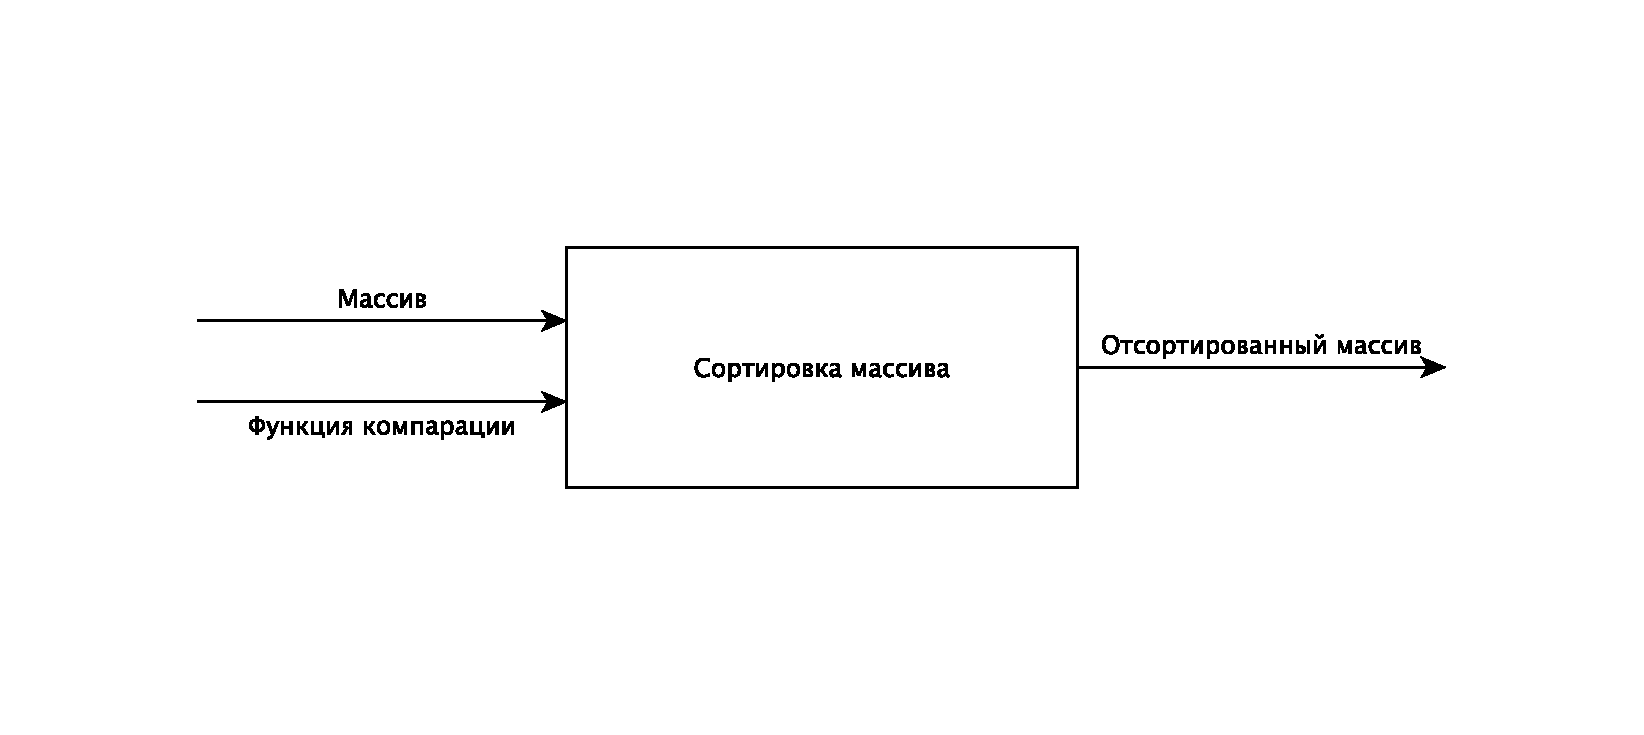
\includegraphics[scale=0.8]{IDEF0}}
    \caption{IDEF0}
    \label{img:idef0}
\end{figure}

\subsection{Схемы алгоритмов}

На рисунке \ref{img:modvinograd} изображена схема
алгоритма Винограда.

\begin{figure}[H]
    \center{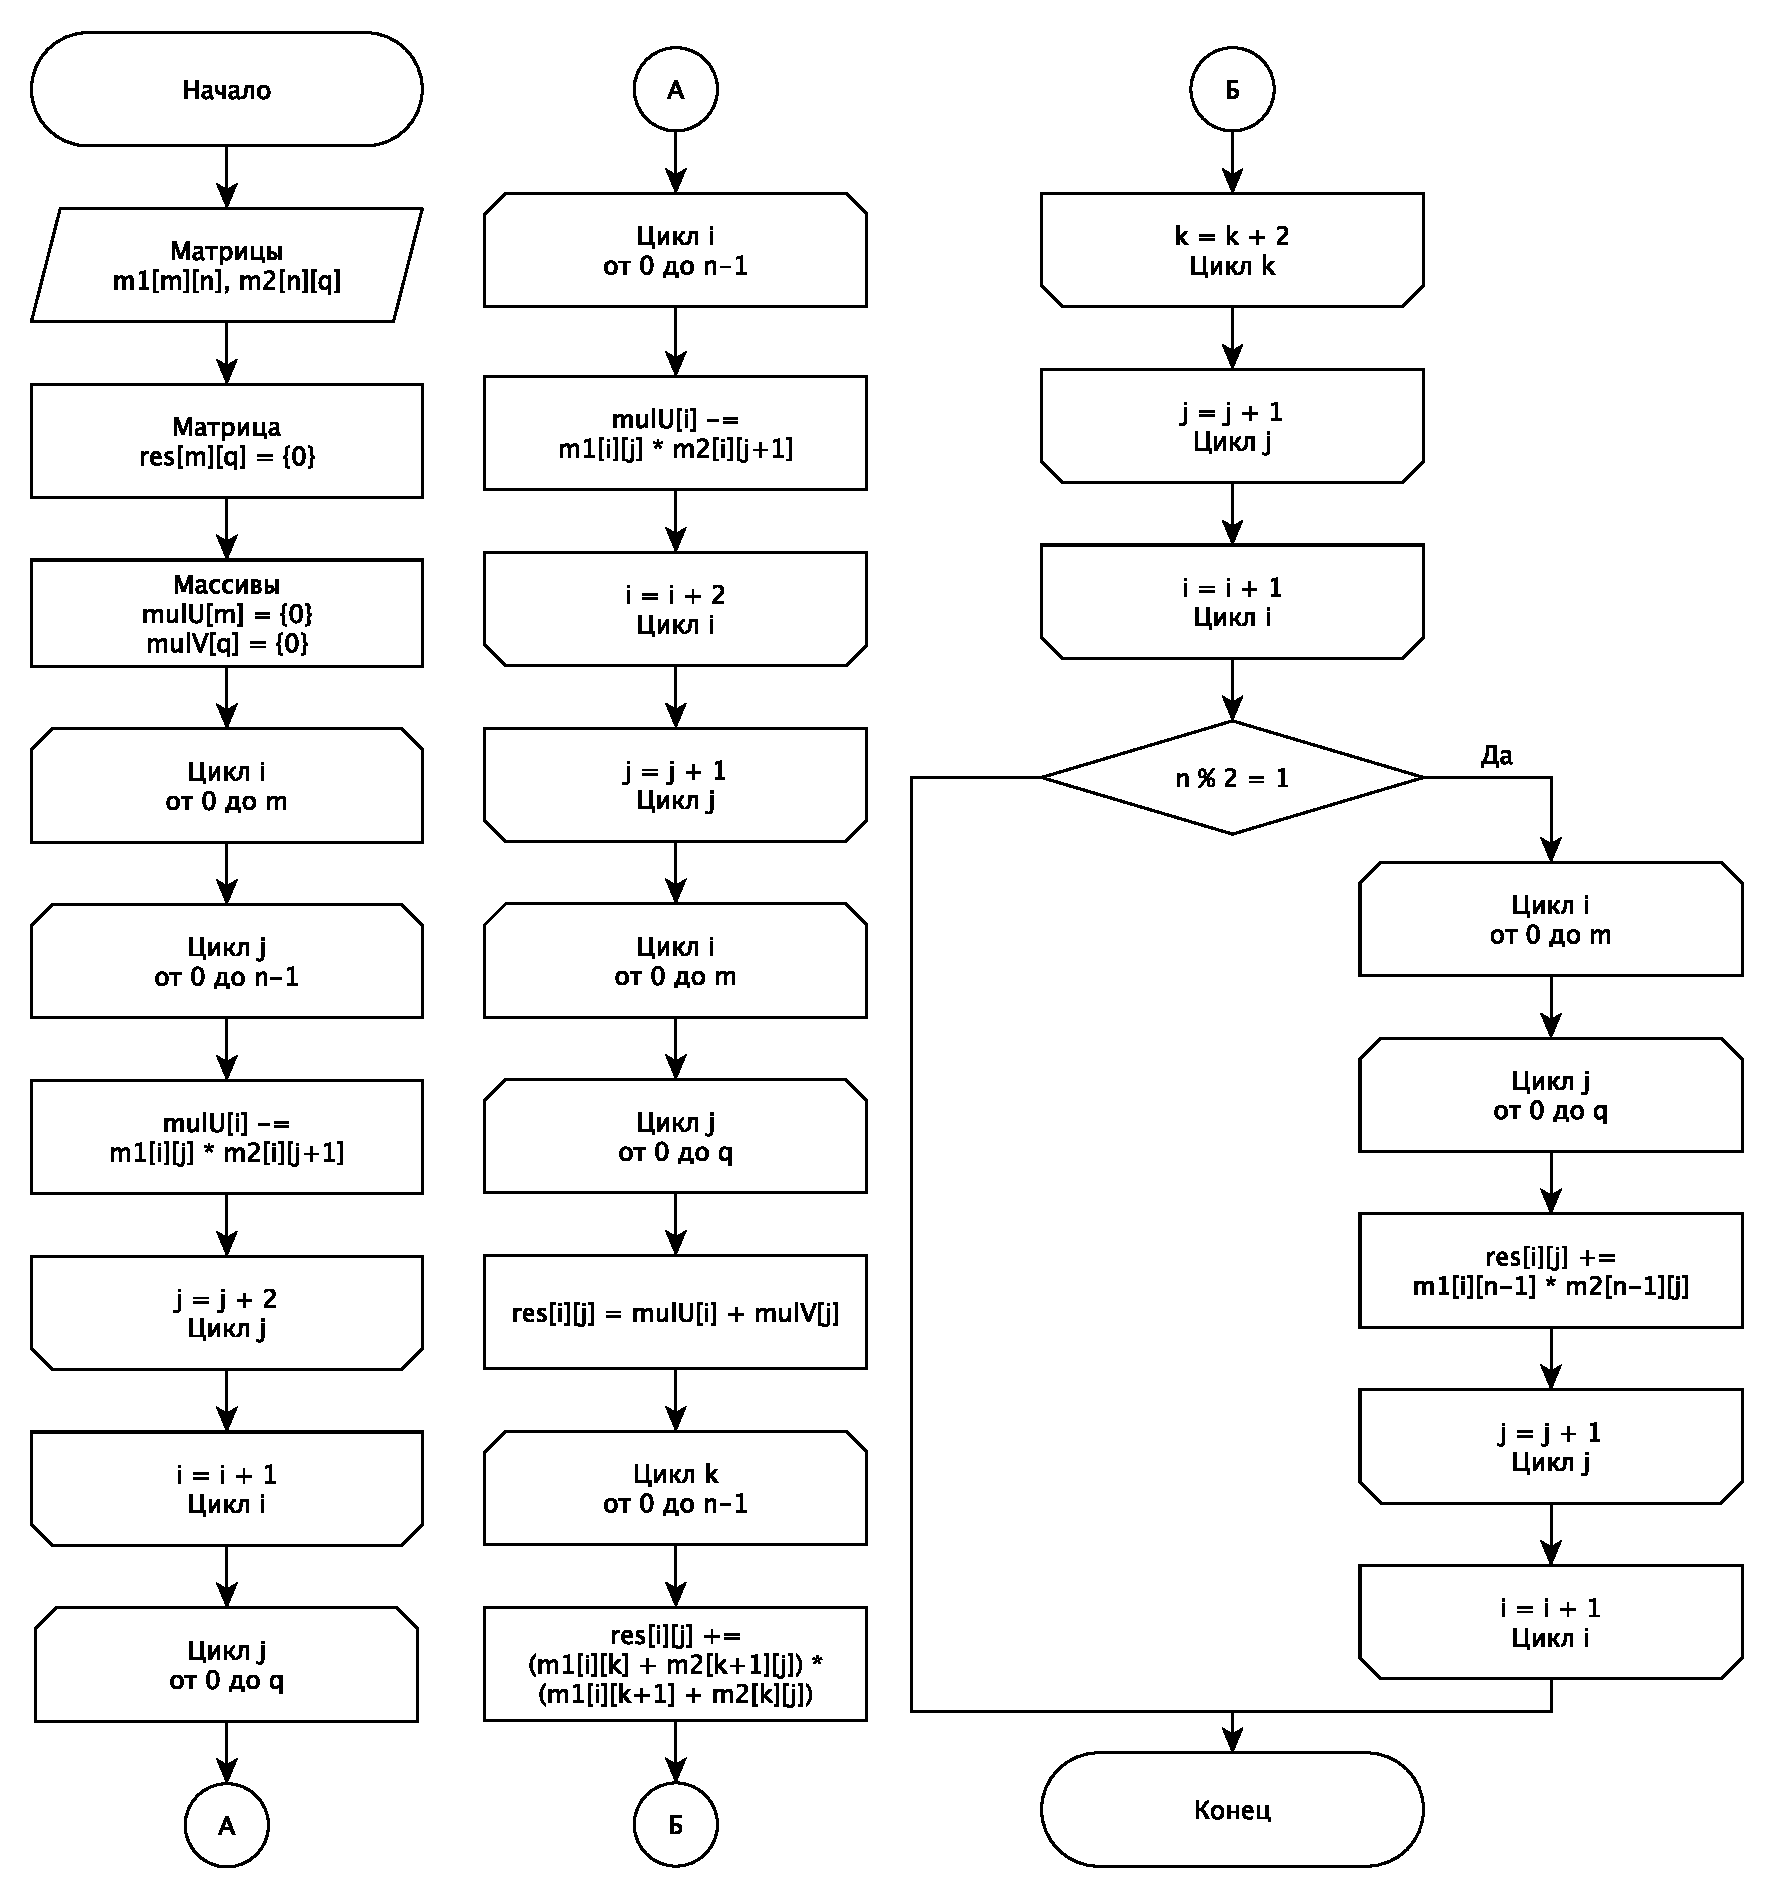
\includegraphics[scale=0.6]{modvinograd}}
    \caption{Схема алгоритма Винограда}
    \label{img:modvinograd}
\end{figure}

На рисунке \ref{img:modvinograd-thread} изображена схема
алгоритма Винограда с возможность распараллеливания вычислений.

\begin{figure}[H]
    \center{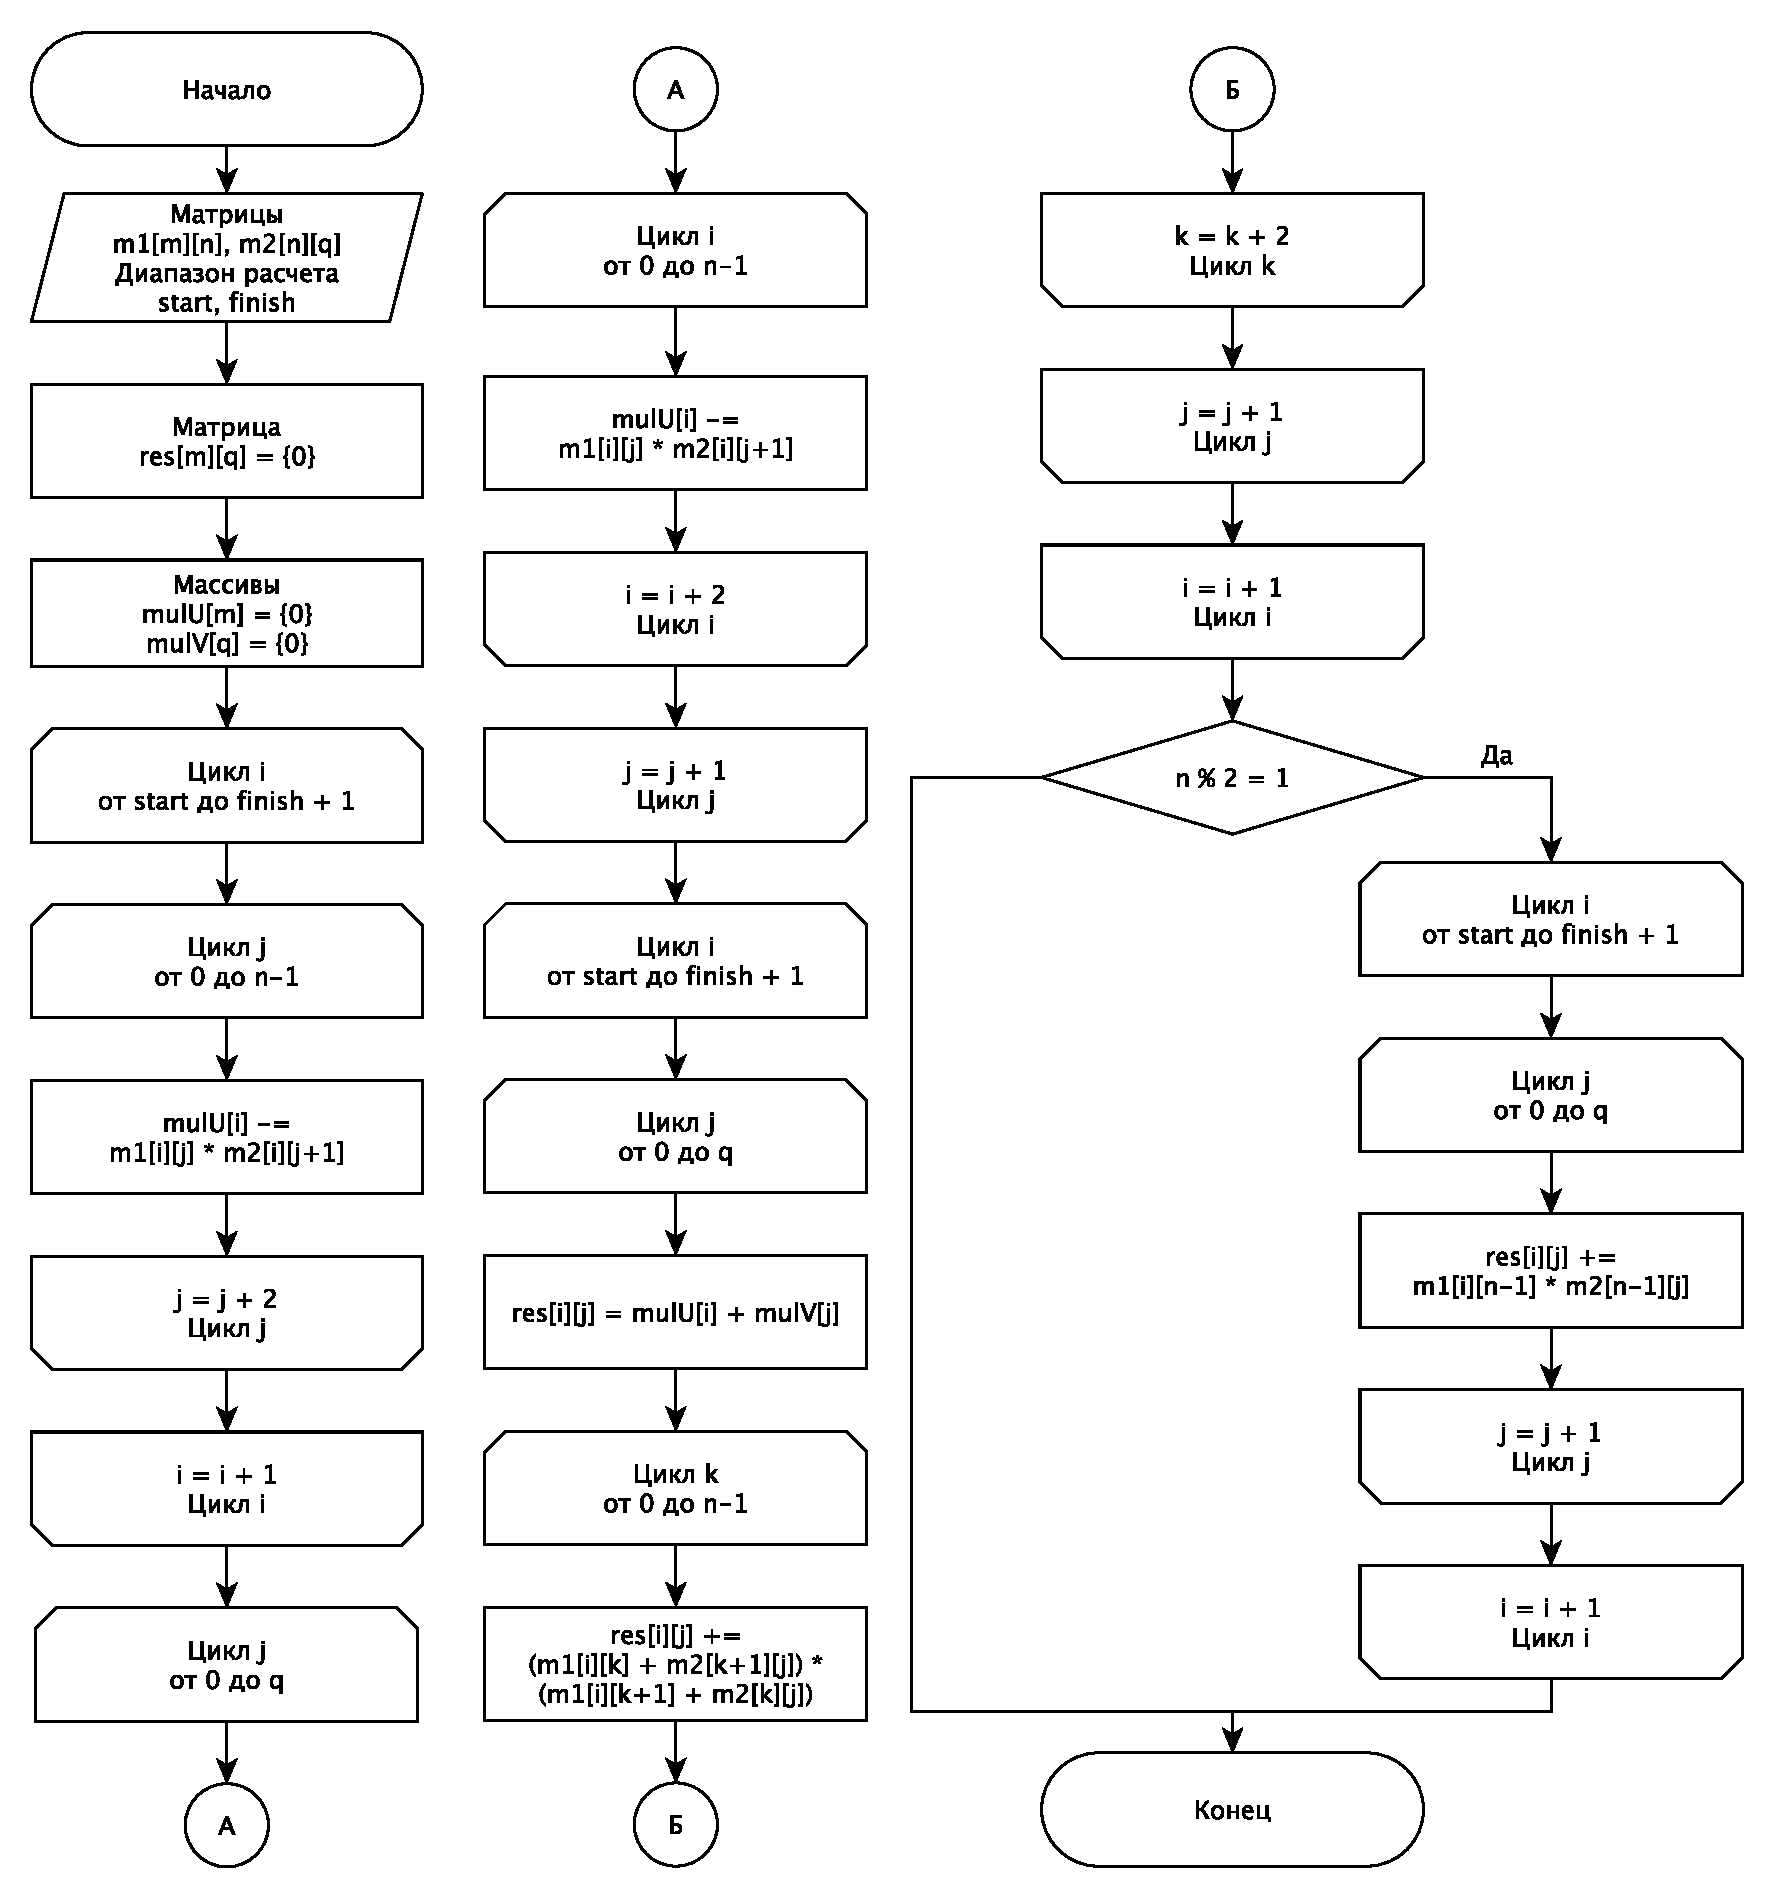
\includegraphics[scale=0.6]{modvinograd_thread}}
    \caption{Схема алгоритма Винограда c возможностью распараллеливания}
    \label{img:modvinograd-thread}
\end{figure}

Распараллеливание вычислений реализовано благодаря добавлению двух новых переменных
{\ttfamily start} и {\ttfamily finish}, которые указывают на диапазон строк, которые
необходимо рассчитать, этот диапазон используется при расчете суммы произведений
{\ttfamily mulU} для строк, а также при расчете результативной матрицы во внешнем цикле, который
отвечает за строки. Передается итоговая матрица с помощью ссылки, что позволяет
одновременно нескольким потокам взаимодействовать с матрицей.

\subsection{Выводы}

Благодаря возможности вычислять каждый элемент результативной матрицы отдельно друг от друга,
удалось разделить вычисления по строчкам, выдавая каждому потоку диапазон строк, в которых
необходимо считать. После выполнения всех потоков и соответственно расчета всех строк матрицы,
получается правильный результат.

\newpage
\section{Технологическая часть}

Необходимо выбрать средства для разработки алгоритмов и подготовить тесты.

\subsection{Требования к программному обеспечению}

Программное обеспечение должно обеспечивать замер процессорного времени выполнения
каждого алгоритма. Проводятся замеры для случайно генерируемых квадратных матриц
размерности до 1000.

\subsection{Средства реализации}

В качестве языка программирования был выбран {\ttfamily C++}.
Данный язык имеет высокую скорость и богатую стандартную библиотеку,
содержащую необходимые контейнеры для данной работы. Программа, написанная на
{\ttfamily C++}, будет доступна на всех платформах.

Время замерялось с помощью библиотеки {\ttfamily chrono}, которая измеряет
процессорное время \cite{chrono}. Для распараллеливания вычислений была
использована библиотека с классом нативных потоков
{\ttfamily std::thread} \cite{thread}.

\subsection{Листинг кода}

Результаты разработки указаны на листингах \ref{list:vin}, \ref{list:vinth}.

\begin{lstlisting}[caption=Алгоритм Винограда умножения матриц,label=vin]
Matrix ModifiedVinogradMultiplication::multiplication(
    const Matrix& first,
    const Matrix& second)
{
    Matrix result;
    if (first[0].size() != second.size()) return result;
    result = CreateMatrix(first.size(), second[0].size(), 0);

    const int m = first.size();
    const int n = second.size();
    const int q = second[0].size();

    Array mulU = CreateArray(m);
    Array mulV = CreateArray(q);

    for (int i = 0; i < m; ++i)
        for (int j = 0; j < n - 1; j += 2)
            mulU[i] -=
                first[i][j] * first[i][j + 1];

    for (int j = 0; j < q; ++j)
        for (int i = 0; i < n - 1; i += 2)
            mulV[j] -=
                second[i][j] * second[i + 1][j];

    for (int i = 0; i < m; ++i) {
        for (int j = 0; j < q; ++j) {
            result[i][j] = mulU[i] + mulV[j];
            for (int k = 0; k < n - 1; k += 2) {
                result[i][j] +=
                    (first[i][k] + second[k + 1][j]) *
                    (first[i][k + 1] + second[k][j]);
            }
        }
    }

    if (n % 2 == 1)
        for (int i = 0; i < m; ++i)
            for (int j = 0; j < q; ++j)
                result[i][j] +=
                    first[i][n - 1] * second[n - 1][j];

    return result;
}
\end{lstlisting}

\begin{lstlisting}[caption=Алгоритм Винограда умножения матриц,label=vinth]
void ThreadMultiplication::multiplication(
    const Matrix& first, const Matrix& second,
    Matrix& result,
    const int start, const int finish)
{
    const int m = first.size();
    const int n = second.size();
    const int q = second[0].size();

    Array mulU = CreateArray(m);
    Array mulV = CreateArray(q);

    for (int i = start; i <= finish; ++i)
        for (int j = 0; j < n - 1; j += 2)
            mulU[i] -=
                first[i][j] * first[i][j + 1];

    for (int j = 0; j < q; ++j)
        for (int i = 0; i < n - 1; i += 2)
            mulV[j] -=
                second[i][j] * second[i + 1][j];

    for (int i = start; i <= finish; ++i) {
        for (int j = 0; j < q; ++j) {
            result[i][j] = mulU[i] + mulV[j];
            for (int k = 0; k < n - 1; k += 2) {
                result[i][j] +=
                    (first[i][k] + second[k + 1][j]) *
                    (first[i][k + 1] + second[k][j]);
            }
        }
    }

    if (n % 2 == 1)
        for (int i = start; i <= finish; ++i)
            for (int j = 0; j < q; ++j)
                result[i][j] +=
                    first[i][n - 1] * second[n - 1][j];
}
\end{lstlisting}

\subsection{Тестирование}

Для тестирования программы были заготовлены следующие тесты на таблице
\ref{table:test}.

\begin{table}[H]
    \caption{Тесты для алгоритмов}
    \label{table:test}
    \centering
    \begin{tabular}{|c|c|c|}
        \hline
        Первая матрца & Вторая матрица & Ожидаемый результат \\
        \hline
        1 2 & 1 2 & \ 7 10 \\
        3 4 & 3 4 & 15 22 \\
        \hline
        1 2 3 & 1 2 3 & \ 30\ \ 36\ \ 42 \\
        4 5 6 & 4 5 6 & \ 66\ \ 81\ \ 96 \\
        7 8 9 & 7 8 9 & 102 126 150 \\
        \hline
        1 2 3 & 1 & 14 \\
        4 5 6 & 2 & 32 \\
              & 3 & \\
        \hline
    \end{tabular}
\end{table}

\subsection{Выводы}

Для сравнения были реализованы 3 алгоритма на выбранном языке
программирования {\ttfamily C++}. Чтобы проверить правильность работы алгоритмов
были подготовлены тесты.

\newpage
\section{Экспериментальная часть}

Проведем тестирование и сравним алгоритмы по времени работы.

\subsection{Примеры работ}

Ниже приведены примеры работ при корректных и некорректных данных

\begin{figure}[H]
    \centering
    \includegraphics[scale=0.5]{zero_arg}
    \caption{Без аргументов}
    \label{img:zero-arg}
\end{figure}

\begin{figure}[H]
    \centering
    \includegraphics[scale=0.5]{less_zero}
    \caption{Некорректный аргумент}
    \label{img:less-arg}
\end{figure}

\begin{figure}[H]
    \centering
    \includegraphics[scale=1]{five}
    \caption{Работа 2 потоков}
    \label{img:five}
\end{figure}

\begin{figure}[H]
    \centering
    \includegraphics[scale=0.6]{ten}
    \caption{Работа 5 потоков}
    \label{img:ten}
\end{figure}

\subsection{Результаты тестирования}

Для тестирования были использованы тесты из таблицы \ref{table:test}.
Результаты продемонстрированы на таблицах \ref{table:test-res} и \ref{table:test-res-th}.

\begin{table}[H]
    \caption{Результаты однопоточного алгоритма}
    \label{table:test-res}
    \centering
    \begin{tabular}{|c|c|c|}
        \hline
        Первая матрца & Вторая матрица & Результат \\
        \hline
        1 2 & 1 2 & \ 7 10 \\
        3 4 & 3 4 & 15 22 \\
        \hline
        1 2 3 & 1 2 3 & \ 30\ \ 36\ \ 42 \\
        4 5 6 & 4 5 6 & \ 66\ \ 81\ \ 96 \\
        7 8 9 & 7 8 9 & 102 126 150 \\
        \hline
        1 2 3 & 1 & 14 \\
        4 5 6 & 2 & 32 \\
              & 3 & \\
        \hline
    \end{tabular}
\end{table}

\begin{table}[H]
    \caption{Результаты многопоточного алгоритма}
    \label{table:test-res-th}
    \centering
    \begin{tabular}{|c|c|c|}
        \hline
        Первая матрца & Вторая матрица & Результат \\
        \hline
        1 2 & 1 2 & \ 7 10 \\
        3 4 & 3 4 & 15 22 \\
        \hline
        1 2 3 & 1 2 3 & \ 30\ \ 36\ \ 42 \\
        4 5 6 & 4 5 6 & \ 66\ \ 81\ \ 96 \\
        7 8 9 & 7 8 9 & 102 126 150 \\
        \hline
        1 2 3 & 1 & 14 \\
        4 5 6 & 2 & 32 \\
              & 3 & \\
        \hline
    \end{tabular}
\end{table}  

Все тесты пройдены успешно.

\subsection{Замеры времени}

На рисунке \ref{img:even} представлены результаты замера времени алгоритмов при
четных размерностях, а на рисунке \ref{img:noteven} при нечетных размерностях матриц.
Оба случая прогонялись на квардатных матрицах.

\begin{figure}[H]
    \begin{tikzpicture}
        \begin{axis}[
            legend pos = north west,
            xlabel=Размерность матрицы,
            ylabel=Милисекунды,
            grid = major,
            width = 0.8\paperwidth,
            height = 0.38\paperheight,
            line width = 1
        ]
            \legend{
                1 поток,
                2 потока,
                4 потока,
                8 потоков,
                16 потоков
            };
            \addplot coordinates {
                (100, 14628)
                (200, 116180)
                (300, 438016)
                (400, 1187214)
                (500, 2385626)
                (600, 4243078)
                (700, 6698034)
                (800, 10465285)
                (900, 21069337)
                (1000, 27797876)
            };

            \addplot coordinates {
                (100, 8757)
                (200, 64567)
                (300, 220776)
                (400, 618716)
                (500, 1229652)
                (600, 2113989)
                (700, 3375514)
                (800, 5236305)
                (900, 11378200)
                (1000, 17093862)
            };

            \addplot coordinates {
                (100, 4715)
                (200, 60202)
                (300, 172877)
                (400, 553051)
                (500, 1066518)
                (600, 1929989)
                (700, 3044136)
                (800, 4601543)
                (900, 8663647)
                (1000, 14690104)
            };

            \addplot coordinates {
                (100, 7619)
                (200, 45675)
                (300, 174078)
                (400, 469850)
                (500, 1036757)
                (600, 1803543)
                (700, 2952666)
                (800, 4592266)
                (900, 7127271)
                (1000, 13610609)
            };

            \addplot coordinates {
                (100, 9139)
                (200, 32580)
                (300, 151308)
                (400, 433387)
                (500, 944650)
                (600, 1666263)
                (700, 3051969)
                (800, 4548904)
                (900, 8071541)
                (1000, 12539912)
            };
        \end{axis}
    \end{tikzpicture}
    \caption{Четная размерность}
    \label{img:even}
\end{figure}

\begin{figure}[H]
    \begin{tikzpicture}
        \begin{axis}[
            legend pos = north west,
            xlabel=Размерность матрицы,
            ylabel=Милисекунды,
            grid = major,
            width = 0.8\paperwidth,
            height = 0.38\paperheight,
            line width = 1
        ]
            \legend{
                1 поток,
                2 потока,
                4 потока,
                8 потоков,
                16 потоков
            };

            \addplot coordinates {
                (101, 15213)
                (201, 117837)
                (301, 443410)
                (401, 1220647)
                (501, 2392950)
                (601, 4218498)
                (701, 6738488)
                (801, 10540792)
                (901, 18951786)
                (1001, 28697609)
            };

            \addplot coordinates {
                (101, 8774)
                (201, 59229)
                (301, 224074)
                (401, 628244)
                (501, 1219904)
                (601, 2159161)
                (701, 3455919)
                (801, 5280501)
                (901, 10318001)
                (1001, 16102750)
            };

            \addplot coordinates {
                (101, 9212)
                (201, 58437)
                (301, 207268)
                (401, 538472)
                (501, 1048101)
                (601, 1907731)
                (701, 2988553)
                (801, 4593652)
                (901, 8808202)
                (1001, 14225764)
            };

            \addplot coordinates {
                (101, 8624)
                (201, 41359)
                (301, 129048)
                (401, 464942)
                (501, 1025854)
                (601, 1799975)
                (701, 2930749)
                (801, 4621777)
                (901, 8195691)
                (1001, 12314462)
            };

            \addplot coordinates {
                (101, 9228)
                (201, 33492)
                (301, 138411)
                (401, 425481)
                (501, 934565)
                (601, 1746171)
                (701, 3141964)
                (801, 4555403)
                (901, 8106159)
                (1001, 14064880)
            };
        \end{axis}
    \end{tikzpicture}
    \caption{Нечетная размерность}
    \label{img:noteven}
\end{figure}

\subsection{Выводы}

Из графиков отношения размерности матрицы ко времени вычисления видно, что рассчет
на одном потоке работает в 2 раза медленнее вычислений на нескольких потоках.
Среди распараллеленных вычислений видно, что увеличение числа потоков дает
небольшой прирост к скорости примерно на 5\%. Но чем больше потоков используется, тем
этот прирост меньше. На графике с четной размерностью можно заметить, что на 1000
размерности 16 потоков начинают проигрывать по скорости 8 потокам.

\newpage
\anonsection{Заключение}

В ходе данной работы было проведено сравнение расчета произведения матриц на нескольких потоках,
а именно на 1, 2, 4, 8 и 16 и были сделаны следующие выводы:

\begin{itemize}
    \item распараллеленные вычисления эффективней в 2 раза;
    \item исользование числа потоков больше, чем число потоков процессора не дает
        выйгрыша по времени и может даже работать медленнее.
\end{itemize}

Все цели, поставленные на эту работы, были выполнены:

\begin{enumerate}
    \item изучение распараллеливания вычислений и работа с потоками;
    \item реализация распараллеленных вычислений;
    \item экспериментальное сравнение работы алгоритма на разном количестве потоков.
\end{enumerate}

\newpage
\addcontentsline{toc}{section}{Список используемой литературы}

\begin{thebibliography}{}
    \bibitem{haskell} Анисимов Н.С. и Строганов Ю.В. - "Реализация алгоритма умножения матриц по Винограду"
на языке Haskell
    \bibitem{litr} Корн Г., Корн Т. - "Алгебра матриц и матричное исчисление"
    \bibitem{chrono} Документация по chrono [Электронный ресурс]. -
    Режим доступа: http://www.cplusplus.com/reference/chrono/
    Дата обращения: 08.10.2019
    \bibitem{thread} Документация по thread [Электронный ресурс]. -
    Режим доступа: https://ru.cppreference.com/w/cpp/thread/thread
    Дата обращения: 21.10.2019
\end{thebibliography}

\end{document}
